%%%%%%%%%%%%%%%%%%%%%%%%%%%%%%%%%%%%%%%%%
% Last Update: Aaron Hill, July 2018
% 			TTU Atmospheric Science Department
%			aaron.hill@ttu.edu
%%%%%%%%%%%%%%%%%%%%%%%%%%%%%%%%%%%%%%%%%


%%%%%%%%%%%%%%%%%%%%%%%%%%%%%%%%%%%%%%%%%
% This documentclass loads the packages  %
%            setspace                   %
% and                                   %
%           fancyhdr.                   %
% You may have to                        %
% get these if your TeX distribution     %
% doesn't have them.                     %
%%%%%%%%%%%%%%%%%%%%%%%%%%%%%%%%%%%%%%%%%
\documentclass{ttuthes2015}

%%%%%%%%%%%%%%%%%%%%%%%%%%%%%%%%%%%%%%%%%%%%%%
% Include any other add-on  packages you need:%
%%%%%%%%%%%%%%%%%%%%%%%%%%%%%%%%%%%%%%%%%%%%%%
\usepackage{amsmath,amssymb,amsthm,graphicx}
\usepackage{natbib}	       % use for citing notation
\usepackage[nottoc,numbib]{tocbibind}  % include bibliography in table of contents
\usepackage[title,titletoc,header]{appendix}

\usepackage{titlesec}
\setcounter{tocdepth}{3}

\titleformat{\section}{\bfseries\normalsize}{\arabic{chapter}.\arabic{section}}{1em}{}
\titleformat{\subsection}{\normalsize}{\arabic{chapter}.\arabic{section}.\arabic{subsection}}{1em}{}
\titleformat{\subsubsection}{\itshape\normalsize}{\arabic{chapter}.\arabic{section}.\arabic{subsection}.\arabic{subsubsection}}{1em}{}

%%%%%%%%%%%%%%%%%%%%%%%%%%%%%%%%%%
% EDIT  (Running head--  REQUIRED)%
%%%%%%%%%%%%%%%%%%%%%%%%%%%%%%%%%%
\rhead{Texas Tech University, \emph{FirstName MiddleInitial. LastName}, Month Year}

%%%%%%%%%%%%%%%%%%%%%%%%%%%%%%%%%%%%%%%%%%%%%%%
% Uncomment if the grad school doesn't like the%
% line under the  running head:                %
%%%%%%%%%%%%%%%%%%%%%%%%%%%%%%%%%%%%%%%%%%%%%%%
\renewcommand{\headrulewidth}{0pt}

%%%%%%%%%%%%%%%%%%%%%%%%%%%%%%%%%%%%%%%%%%%%%%%%%%%%%
% Following commands add blank space underneath entries in the List of Figures and List of    %
% Tables, per the new grad school requirements. Entries with multiple lines are single spaced. %
% Users will need to add "\addLOFspace" or "\addLOTspace" after their figure or table, respectively. %
%%%%%%%%%%%%%%%%%%%%%%%%%%%%%%%%%%%%%%%%%%%%%%%%%%%%%
\newcommand{\addLOFspace}[1][2ex]{\addtocontents{lof}{\protect\addvspace{#1}}}
\newcommand{\addLOTspace}[1][2ex]{\addtocontents{lot}{\protect\addvspace{#1}}}
\newcommand{\addTOCspace}[1][2ex]{\addtocontents{toc}{\protect\addvspace{#1}}}

%%%%%%%%%%%%%%%%%%%%%%%%%%%%%%%%%%%%%%%%%%%%%%%%%%
%Spacing -- Do you want double or one-and-a-half?%
%%%%%%%%%%%%%%%%%%%%%%%%%%%%%%%%%%%%%%%%%%%%%%%%%%
\doublespacing
%\onehalfspacing

%%%%%%%%%%%%%%%%%%%%%%%%%%%%%%%%%%%%%%%%%%%%%%%%%%%%%%%%%%%%%
%Leave the one you want uncommented.                        %
%In places where single-line-spacing is appropriate         %
%e.g, extended quotations, you can enclose the material     %
%in a singlespacing environment (with \begin{singlespacing} %
% ...  \end{singlespacing}                                  %
%%%%%%%%%%%%%%%%%%%%%%%%%%%%%%%%%%%%%%%%%%%%%%%%%%%%%%%%%%%%%


%%%%%%%%%%%%%%%%%%%%%%%%%%%%%%%%%%%%%%%%%%%%%%%%%%
%Other preamble stuff, e.g., theorem environments%
%or newcommands go here:                         %
% e.g.                                           %
%%%%%%%%%%%%%%%%%%%%%%%%%%%%%%%%%%%%%%%%%%%%%%%%%%
% \newtheorem{theorem}{Theorem}
% \newtheorem{proposition}[theorem]{proposition}
% \newtheorem{question}{Question}
% \newtheorem{conjecture}{Conjecture}
\newcommand{\tab}{\hspace*{2em}}  % tabbing for paragraphs

\bibliographystyle{ametsoc}   % use american meteorological society bibliography style (2014 version)
\bibpunct{(}{)}{;}{a}{}{,}   % set punctuation for citing articles, books, etc. (AMS Style)

\begin{document}

%%%%%%%%%%%%%%%%%%%%%%%%%%%%%%%%%%%%%%%%%%%%%%%%%%%%%%%%
%TITLE PAGE -- Edit the spacing commands after each \\ %
% if necessary                                         %
%%%%%%%%%%%%%%%%%%%%%%%%%%%%%%%%%%%%%%%%%%%%%%%%%%%%%%%%
\begin{titlepage}
\vbox to  \textheight{
\begin{singlespacing}
\begin{center}
"Insert Your Title Here" \\[12pt]  %Edit
by\\[12pt]
FirstName MiddleInitial. LastName, B.S.\\[12pt]   %Edit
A Thesis\\[12pt]   % or Thesis
In\\[12pt]
Atmospheric Science\\[12pt]  % Edit
Submitted to the Graduate Faculty\\
of Texas Tech University in\\
Partial Fulfillment of\\
the Requirements for\\
the Degree of\\[12pt]
MASTERS OF SCIENCES\\[12pt]  %Edit
Approved\\[12pt]
Dr. Committee Chair Name\\ %Edit
Committee Chair\\[12pt]
Dr. Jane Doe\\[12pt] %Edit
Dr. Joe Doe\\[12pt] %Edit
Mark Sheridan\\ %Edit
Dean of the Graduate School\\[12pt]
July, 2020     %Edit
\end{center}
\end{singlespacing}
\vfill}
\end{titlepage}
%%%%%%%%%%%%%%%%%%%
%End of title page%
%%%%%%%%%%%%%%%%%%%

%%%%%%%%%%%%%%%%%%%%%%%%%%%%%%%%%%%%%%%%%%%%%%%%%%%%%%%
%Copyright page -- delete or comment out if not needed%
%usage: \copyrightpage{year of appearance}{Name}      %
%%%%%%%%%%%%%%%%%%%%%%%%%%%%%%%%%%%%%%%%%%%%%%%%%%%%%%%
%\copyrightpage{2020}{FirstName MiddleInitial. LastName} %Name should be same as on
\begin{center}
\vspace*{\fill}
Copyright 2020, John H. Doe
\vspace*{\fill}
\end{center}


%title page
%%%%%%%%%%%%%%%%%%%%%%%%
%\end of copyright page%
%%%%%%%%%%%%%%%%%%%%%%%%

%%%%%%%%%%%%%%%%%%%%%%%
%Start of frontmatter %
%You need this:       %
%%%%%%%%%%%%%%%%%%%%%%%
\frontmatter     % does the numbering and makes new pages


%%%%%%%%%%%%%%%%%%%%%%%%%%%%%
%Acknowledgements           %
%Comment out or delete      %
%if not  wanted             %
%%%%%%%%%%%%%%%%%%%%%%%%%%%%%
\chapter{Acknowledgements}
\addTOCspace
\tab "insert acknowledgement text here"


%%%%%%%%%%%%%%%%%%%%%%%%%
%End of acknowledgements%
%%%%%%%%%%%%%%%%%%%%%%%%%

%%%%%%%%%%%%%%%%%%%
%Table of Contents%
%%%%%%%%%%%%%%%%%%%
\singlespacing
\tableofcontents

%%%%%%%%%%%%%%%%%%%%%%%%%%%%%%%%%%%%%%%%%%%%%%%%%%
%Abstract -- Delete or comment out if not wanted:%
%%%%%%%%%%%%%%%%%%%%%%%%%%%%%%%%%%%%%%%%%%%%%%%%%%
\doublespacing
\chapter{Abstract}
\addTOCspace
\tab "insert abstract text here"


%%%%%%%%%%%%%%%%%
%End of abstract%
%%%%%%%%%%%%%%%%%


%%%%%%%%%%%%%%%%%%%%%%%%%%%%%%%%%%%%%
% List of tables and list of figures %
% Delete or comment out if not needed %
% Single spacing is needed to get the blank space correct. %
%%%%%%%%%%%%%%%%%%%%%%%%%%%%%%%%%%%%%
\singlespacing
\listoftables
\addTOCspace

\listoffigures
\addTOCspace


%%%%%%%%%%%%%%%%%%%%%%%%%%%%%%%%%%%%
%End of lists of tables and figures%
%%%%%%%%%%%%%%%%%%%%%%%%%%%%%%%%%%%%

%%%%%%%% OPTIONAL CHAPTER FOR ABBREVIATIONS %%%%%%%%%%%%%
\doublespacing
\chapter{List of Abbreviations}
\addTOCspace
e.g. \\
F - Fahrenheit \\


%%%%%%%%%%%%%%%%%%%%%%%%%%%%%%%%%%%%%%%%%%%%


%%%%%%%%%%%%%%%%%%%%%%%%
%MAIN PART OF  DOCUMENT%
%%%%%%%%%%%%%%%%%%%%%%%%

\mainmatter

\chapter{Introduction}  % how to make a chapter
\addTOCspace

%Type is: $\@chapapp$

"Intro text"

\section{Section Title}  % how to make a section
\addTOCspace

% figure
\tab Make a figure like this
\begin{figure}[!htb]
  \centering
  \noindent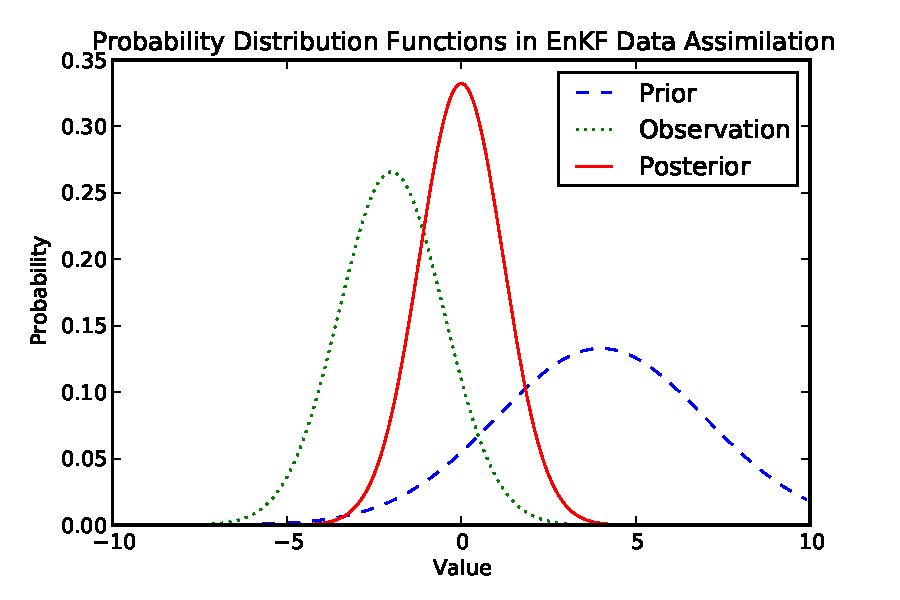
\includegraphics[width=30pc,angle=0]{./example.pdf}\\
     \caption{Example figure caption that is very long and has wrap around text in the list of figures that needs to be single spaced while each individual entry in the list of figures needs to be double spaced.}
\label{example}
\addLOFspace
\end{figure}

\tab Reference a figure: Fig.~$\ref{example}$ \\

\tab Make a figure like this
\begin{figure}[!htb]
  \centering
  \noindent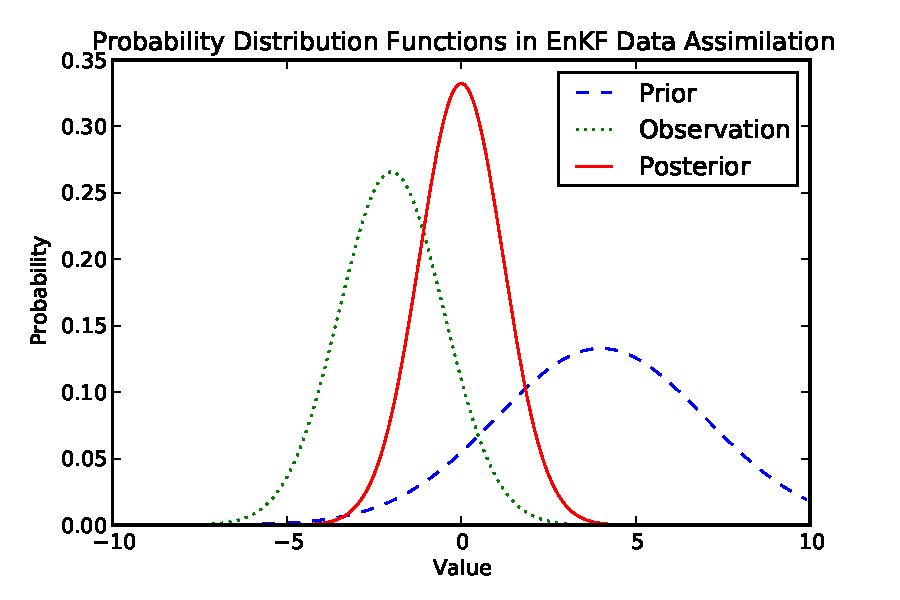
\includegraphics[width=30pc,angle=0]{./example.pdf}\\
  \caption{Example figure and caption}
\label{example2}
\end{figure}

% equation
\tab Make an equation like this
\begin{align}\label{J_var}
	\sigma = \frac{1}{M-1} \delta\bf{J} \delta{\mathbf{J}}^T.
\end{align}

\tab Reference an equation: ($\ref{J_var}$) \\
% citing
\tab Ways to Cite (there are more, google them) \\
\citep{Ancell2013} \\
\cite{Ancell2013} \\

\tab Make a simple table like this
\begin{table}[!h]   % makes it at the instance it is created ! - instantly, h- here, b-bottom, t-top
\caption{Model Parameterizations Used} 
\centering % used for centering table 
\scalebox{0.8}{
\begin{tabular}{c c} % centered columns (1 column) 
\\ [0.5ex] \hline
Parameterization Types & Schemes Used \\ [0.5ex] % inserts table 
%heading 
\hline % inserts single horizontal line 
Boundary Layer & Yonsei University \\ % inserting body of the table 
Cumulus* & Kain-Fritsch \\ % inserting body of the table 
Land Surface & Noah LSM \\ 
Long-Wave Radiation & Rapid Radiative Transfer Model  \\ 
Short-Wave Radiation & Dudhia \\ 
Microphysics & Thompson \\ [1ex] 
\hline %inserts single line 
\end{tabular} 
} \\
*Convection is explicitly resolved on the third domain
\label{params} % is used to refer this table in the text 
\end{table} 


\subsection{Subsection Title} % how to make a subsection
\addTOCspace

\subsubsection{Subsubsection title}
\addTOCspace

%%%%%%%%%%%%%%%%%%%%%%%%%%%%%%%%%%%%%%%%%%%%%%
%Backmatter -- Bibliography, appendices, etc.%
%%%%%%%%%%%%%%%%%%%%%%%%%%%%%%%%%%%%%%%%%%%%%%
\backmatter


%%%%%%%%%%%%%%%%%%%%%%%%%%%%%%%%%%%%%%%%%%%%%%%%%%%%%%%%
%Bibliography:  Use BibTeX if you like. Or enter the items in directly with correct formatting. %
%%%%%%%%%%%%%%%%%%%%%%%%%%%%%%%%%%%%%%%%%%%%%%%%%%%%%%%%

\singlespacing
\bibliography{thesis}

%%%%%%%%%%%%%%%%%%%%%%%%%%%%%%%%%%%%%%%%%%%%%%%%%%%%%%%%
% NOTE: There are small issues with bibliography entry ordering. Edits have to be made in the *.bbl file to align multiple authors correctly
%%%%%%%%%%%%%%%%%%%%%%%%%%%%%%%%%%%%%%%%%%%%%%%%%%%%%%%%


%\begin{thebibliography}{99}   % use when bibtex is not

%%%%%%%%%% EXAMPLE BIB ENTRY TYPED OUT WITHOUT BIBTEX %%%%%%%%%%%%%%
%Ancell, B., and G. J. Hakim, 2007: \emph{Comparing adjoint- and ensemble-sensitivity analysis with applications to observation targeting}. Mon. Wea. Rev., 135, 411--4134.
%\newline\newline
%%%%%%%%%%%%%%%%%%%%%%%%%%%%%%%%%%%%%%%%%%%%%%%%%%%%

%\end{thebibliography}

%%%%%%%%%%%%%%%%%%%%%%%%%%%%%%%%%%%%%%%%%%%%%
%If there's only one appendix, just call it %
%"Appendix".  Otherwise, use "Appendix A",  %
%"Appendix B", etc.                         %
%%%%%%%%%%%%%%%%%%%%%%%%%%%%%%%%%%%%%%%%%%%%%

%\appendix
%
%\addtocontents{toc}{\protect\setcounter{tocdepth}{0}}   % don't remove, prevents sections from being added to TOC
%\section*{Appendices} % don't remove, sections are lettered in appendices
%
%\chapter{Appendix A}
%
%%%%%%%%%%%%%%%%%%%%%%%%%%%%%%%%%%%%%%%%%%%%%%%%%%
%\setcounter{figure}{0}   % set figure, table, and section counters to 0 for correct numbering
%\setcounter{table}{0}
%\setcounter{section}{0}
%\renewcommand{\thefigure}{A.\arabic{figure}}
%\renewcommand{\thesection}{A.\arabic{section}}
%%%%%%%%%%%%%%%%%%%%%%%%%%%%%%%%%%%%%%%%%%%%%%%%%%
%
%\section{First Section Title}
%\section{Second Section Title}
%\section{Third Section Title}
%
%% Some computer code
%\begin{singlespacing}
%\begin{verbatim}
%#include <iostream>
%
%using namespace std;
%
%int main(){
%   cout << "Hello world!\n";
%   return  0;
%}
%\end{verbatim}
%\end{singlespacing}
%
%
%
%\chapter{Appendix B}
%
%%%%%%%%%%%%%%%%%%%%%%%%%%%%%%%%%%%%%%%%%%%%%%%%%%
%\setcounter{figure}{0}
%\setcounter{table}{0}
%\setcounter{section}{0}
%\renewcommand{\thefigure}{B.\arabic{figure}}
%\renewcommand{\thesection}{B.\arabic{section}}
%%%%%%%%%%%%%%%%%%%%%%%%%%%%%%%%%%%%%%%%%%%%%%%%%%
%
%\section{First Section Title}
%\section{Second Section Title}
%\section{Third Section Title}
%
%% extra figures to include
%\begin{figure}[!htb]
%  \centering
%  \noindent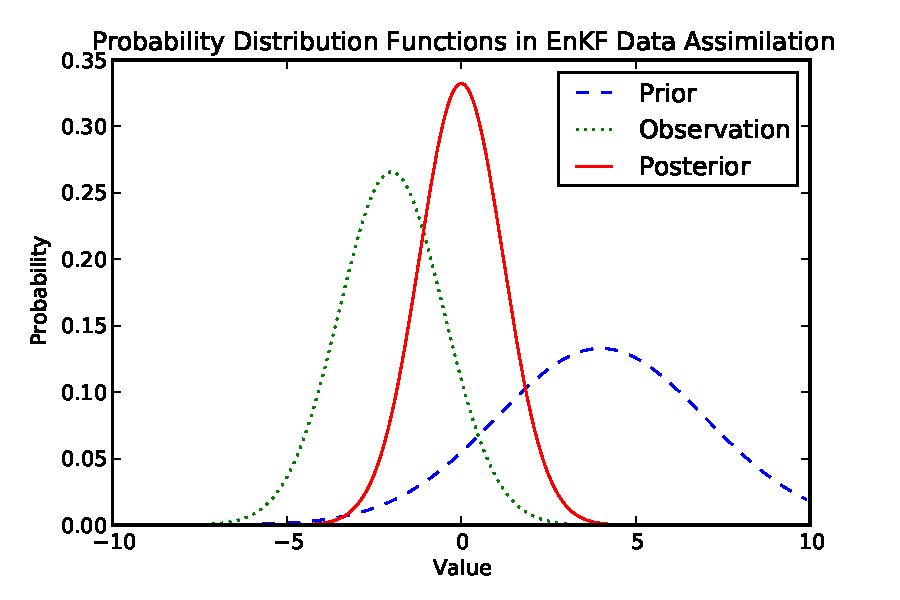
\includegraphics[width=30pc,angle=0]{./example.pdf}\\
%  \caption{Example figure and caption}
%\end{figure}
%
%\begin{figure}[!htb]
%  \centering
%  \noindent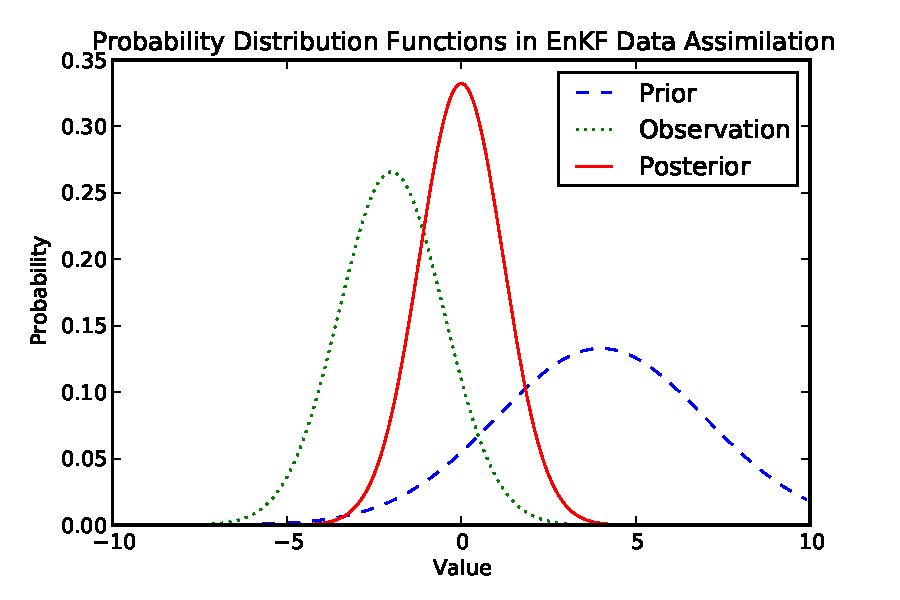
\includegraphics[width=30pc,angle=0]{./example.pdf}\\
%  \caption{Example figure and caption}
%\end{figure}
%
%% if additional appendices are needed, copy the beginning commands and change appropriate lettering to accommodate 
%

\end{document}


 
